\documentclass{standalone}
\usepackage{tikz}
\usepackage{ctex,siunitx,bm}
\setCJKmainfont{Noto Serif CJK SC}
\usepackage{tkz-euclide}
\usepackage{amsmath}
\usetikzlibrary{patterns, calc}
\usetikzlibrary {decorations.pathmorphing, decorations.pathreplacing, decorations.shapes,}
\begin{document}
\small
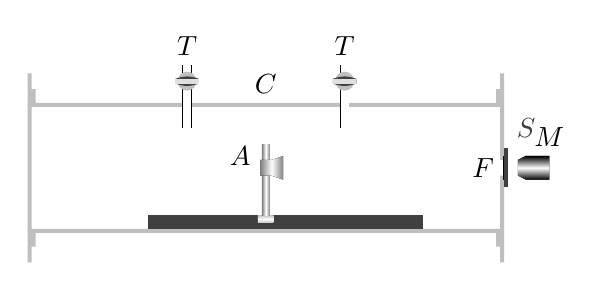
\begin{tikzpicture}[>=latex,scale=1.0]
  \draw[lightgray,line width=0.5mm](-3,1.2)--(-3,-1.2)(3,1.2)--(3,0.1)(3,-1.2)--(3,-0.1)(-2.95,1.0)--++(0,-0.2)--(-1.05,0.8)(-0.95,0.8)--(0.95,0.8)node[midway,above,text=black]{$C$}(1.05,0.8)--(2.95,0.8)--++(0,0.2)(-2.95,-1.0)--++(0,0.2)--++(5.9,0)--++(0,-0.2);
  \fill[darkgray](-1.5,-0.775)rectangle(2,-0.6);
  \fill[top color=lightgray,bottom color=lightgray, middle color=white](-0.1,-0.6)rectangle(0.1,-0.7);
  \fill[left color=gray,right color=gray, middle color=white](-0.05,-0.6)rectangle(0.05,0.3);
  \fill[left color=gray,right color=gray, middle color=white](-0.07,0.1)--(0.07,0.1)--++(0.15,0.05)--++(0,-0.3)--++(-0.15,0.05)--++(-0.14,0)node[above left]{$A$}--cycle;
  \draw[thick](3.03,-0.15)--++(0,0.3)node[midway,left]{$F$};
  \draw[darkgray,very thick](3.05,-0.25)--++(0,0.5)node[above right]{$S$};
  \fill[top color=black,bottom color=black, middle color=white]
  (3.2,0.1)--++(0.1,0.05)--++(0.3,0)node[above]{$M$}--++(0,-0.3)--++(-0.3,0)--++(-0.1,0.05)--cycle;
  \foreach \x in {-1,1}
  {
    \draw[line width=0.1mm,double,double distance=1mm](\x,0.5)--++(0,0.8)node[above]{$T$};
    \fill[lightgray](\x,1.1)circle(0.12);
    \fill[darkgray](\x-0.15,1.07)to[bend right=20](\x+0.15,1.07)--(\x+0.15,1.13)to[bend right=20](\x-0.15,1.13);
    \fill[lightgray!50](\x-0.15,1.07)rectangle(\x+0.15,1.13);
  }
\end{tikzpicture}
\end{document}